\newpage
\section{Consuntivo Finale} \label{Consuntivo Finale}

In questa sezione viene presentato il consuntivo finale del progetto. Gli scostamenti rispetto al \hyperref[Preventivo]{preventivo iniziale} sono derivati dal consuntivo dei periodi analizzati precedentemente e dalle modifiche alla pianificazione. Viene inoltre riportata la suddivisione delle ore fra i componenti del gruppo. \\
In questa sezione verrà preso in considerazione solo il preventivo per i periodi a carico del committente.

\subsection{Preventivo finale}
\begin{table}[h!]
	\centerline{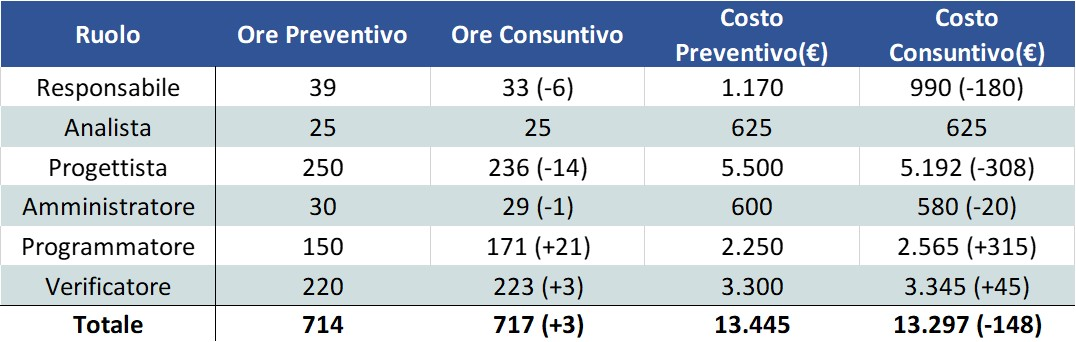
\includegraphics[scale=0.60]{img/Preventivo/Consuntivo/PreventivoFinire.jpg}}
	\caption{Preventivo finale}
\end{table}

Nel seguente grafico è possibile visualizzare l'impegno percentuale per ogni ruolo.

\begin{table}[h!]
	\centerline{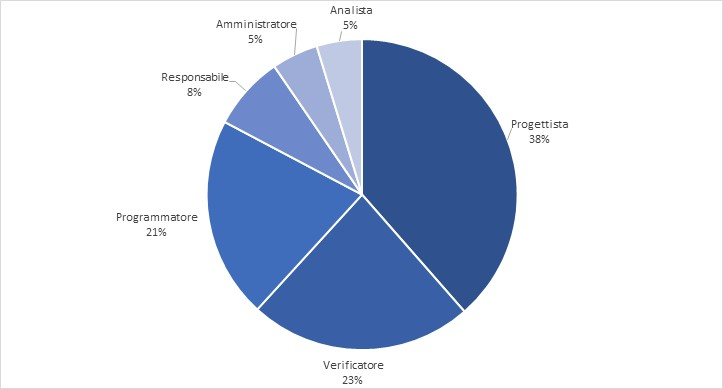
\includegraphics[scale=0.80]{img/Preventivo/Torte/PreventivoFinire.jpg}}
	\caption{Raffigurazione Preventivo finale}
\end{table}

\newpage
\subsection{Ripartizione ore finale}
\begin{table}[h!]
	\centerline{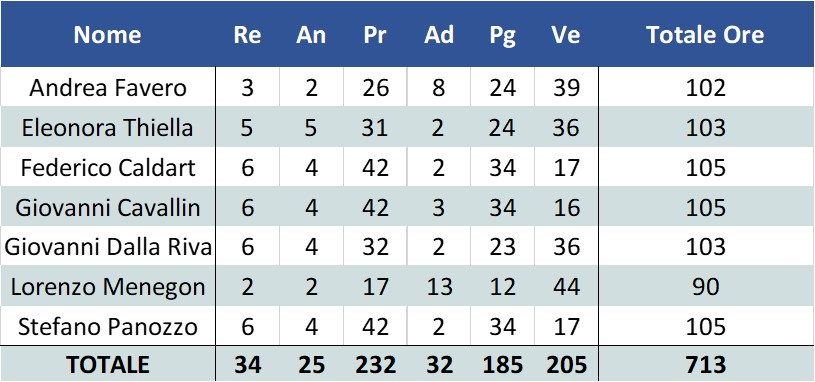
\includegraphics[scale=0.60]{img/Preventivo/Consuntivo/TotaleOre.jpg}}
	\caption{Ripartizione ore finale}
\end{table}

Nel seguente grafico è possibile visualizzare l'impegno individuale dei componenti del gruppo.

\begin{table}[h!]
	\centerline{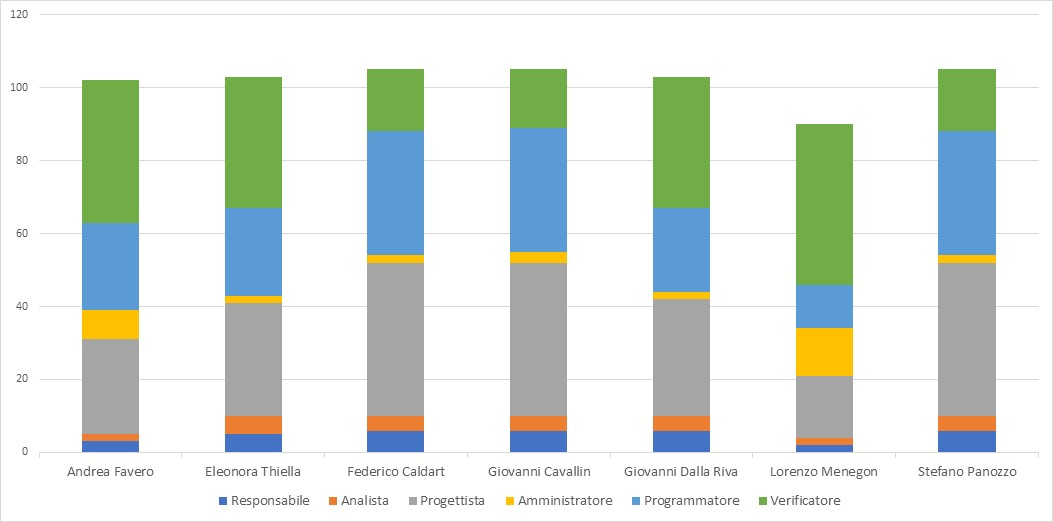
\includegraphics[scale=0.55]{img/Preventivo/Istogrammi/TotaleOre.jpg}}
	\caption{Raffigurazione Ripartizione ore finale}
\end{table}

\subsection{Conclusioni}
Rispetto al preventivo iniziale, sono state effettuate alcune modifiche dovute agli scostamenti rilevati nei vari consuntivi di periodo relativi. A seguito di questi, si è realizzato un impegno significativamente minore per i \progs{} ed i \vers{}, mentre, in contrapposizione, un impegno maggiore per i \progrs{}. Nel complesso il costo totale rendicontato finale risulta \EUR{13.239}, con un risparmio pari a \EUR{206} per il committente rispetto a quanto preventivato inizialmente.
